\subsubsection*{Problem definition}

The aim of this example is to simulate the solute transport in an aquifer by convection with the influence of retardation as a result of sorption. The solute transport is influenced by linear sorption processes. That means, the Henry-isotherm is relevant to calculate the solute concentration. The calculation area and boundary conditions are the same as described for the precedent example.

\textsl{Assumptions}

\begin{tabbing}
Component: \= exclusively linear sorption (Henry isotherm), no decay \\
Aquifer: \> homogeneous, saturated, stationary flow \\
\end{tabbing}

\subsubsection*{Model set-up of the 1~D numerical model}

See chapter \ref{sec:decay}.

The soil parameters are the same as listed in table \ref{tab51}, but decay is not considered during these simulation runs. For the different simulation runs the Henry-sorption coefficients are varied as listed in table \ref{tab52} in order to evaluate the influence of sorption on the mass transport. The retardation coefficients R are calculated by solving equation \ref{eq52}.

\begin{table}[htbp]
\centering
\begin{tabular}{|l|l|}
\hline
K$_D$-value [m$^3$/kg] & retardation coefficient [-] \\
\hline
0  & 1  \\			
\hline
6.8 $\cdot 10^{-6}$ & 1.05 \\
\hline
6.8 $\cdot 10^{-5}$ & 1.54  \\
\hline
6.8 $\cdot 10^{-4}$ & 6.44  \\
\hline
\end{tabular}
\caption{Variation of K$_D$-values and retardation coefficients as input variables}
\label{tab52}
\end{table}

\subsubsection*{Evaluation method}

The concentration distribution at a special point in time and over a given distance is calculated by equation \ref{eq53}. Hereby the decay term $\gamma$ is set equal to 1. The analytical solutions are depicted in figure \ref{fig53} as single symbols.

\subsubsection*{Results}

In figure \ref{fig53} you can find the concentration distribution over the whole length of the 1~D model at the final simulation time of 100 days. Obviously, the numerical results meet well the analytical solutions.


\begin{figure}[htbp]
\centering
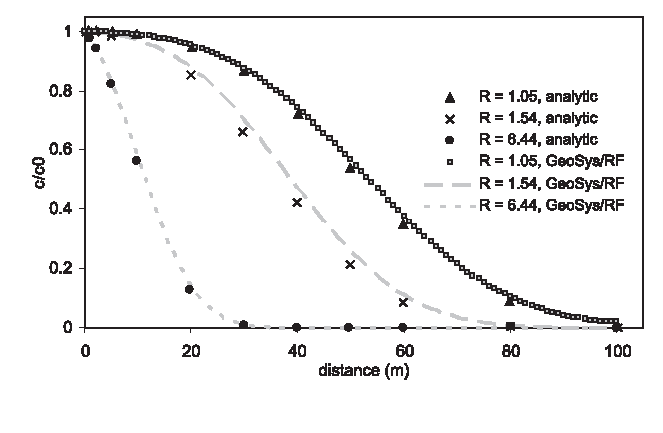
\includegraphics[width=0.8\textwidth]{C/figures/fig53.eps}
\caption{Concentration distribution after 100~d (Henry sorption)}
\label{fig53}
\end{figure}

\begin{tabular}{|l|l|l|}
\hline
Benchmark & Problem type	& Path in benchmark deposit \\
\hline	
hc\_sorp\_henry\_1D	& HC	& benchmarks $\backslash$HC$\backslash$Sorption$\backslash$Henry \\
\hline	
\end{tabular}
